\chapterpage{System Design and Architecture}
\mychapter{System Design and Architecture}
\label{chap:sysdesign}

The architecture and design of the proposed system are documented in this chapter. Starting at the topmost level of architecture, the chapter goes through increasingly detailed structural and behavioural depictions of the system, ending with a proposed logical data model for storing run results beyond the current session.

\section{System Architecture Overview}

The system has a layered, pipe-and-filter architecture: A fixed sequence of processing stages (``filters'') with well defined data flows (``pipes'') between them, each stage contains a single purpose interface for communicating with neighbouring stages. This style was selected to avoid having to deploy multiple instances of the same operator at the same time horizontally across multiple machines and/or CPU cores, and because the work could be considered a linear transformation chain (raw frame~$\rightarrow$~enhanced frame~$\rightarrow$~detections/density~$\rightarrow$~fused count~$\rightarrow$~annotated output), which is a workload type that is not supported by either of the other options.

The five architectural layers can be pinpointed as follows (see Figure~\ref{fig:archoverview}):

\begin{figure}[H]
    \centering
    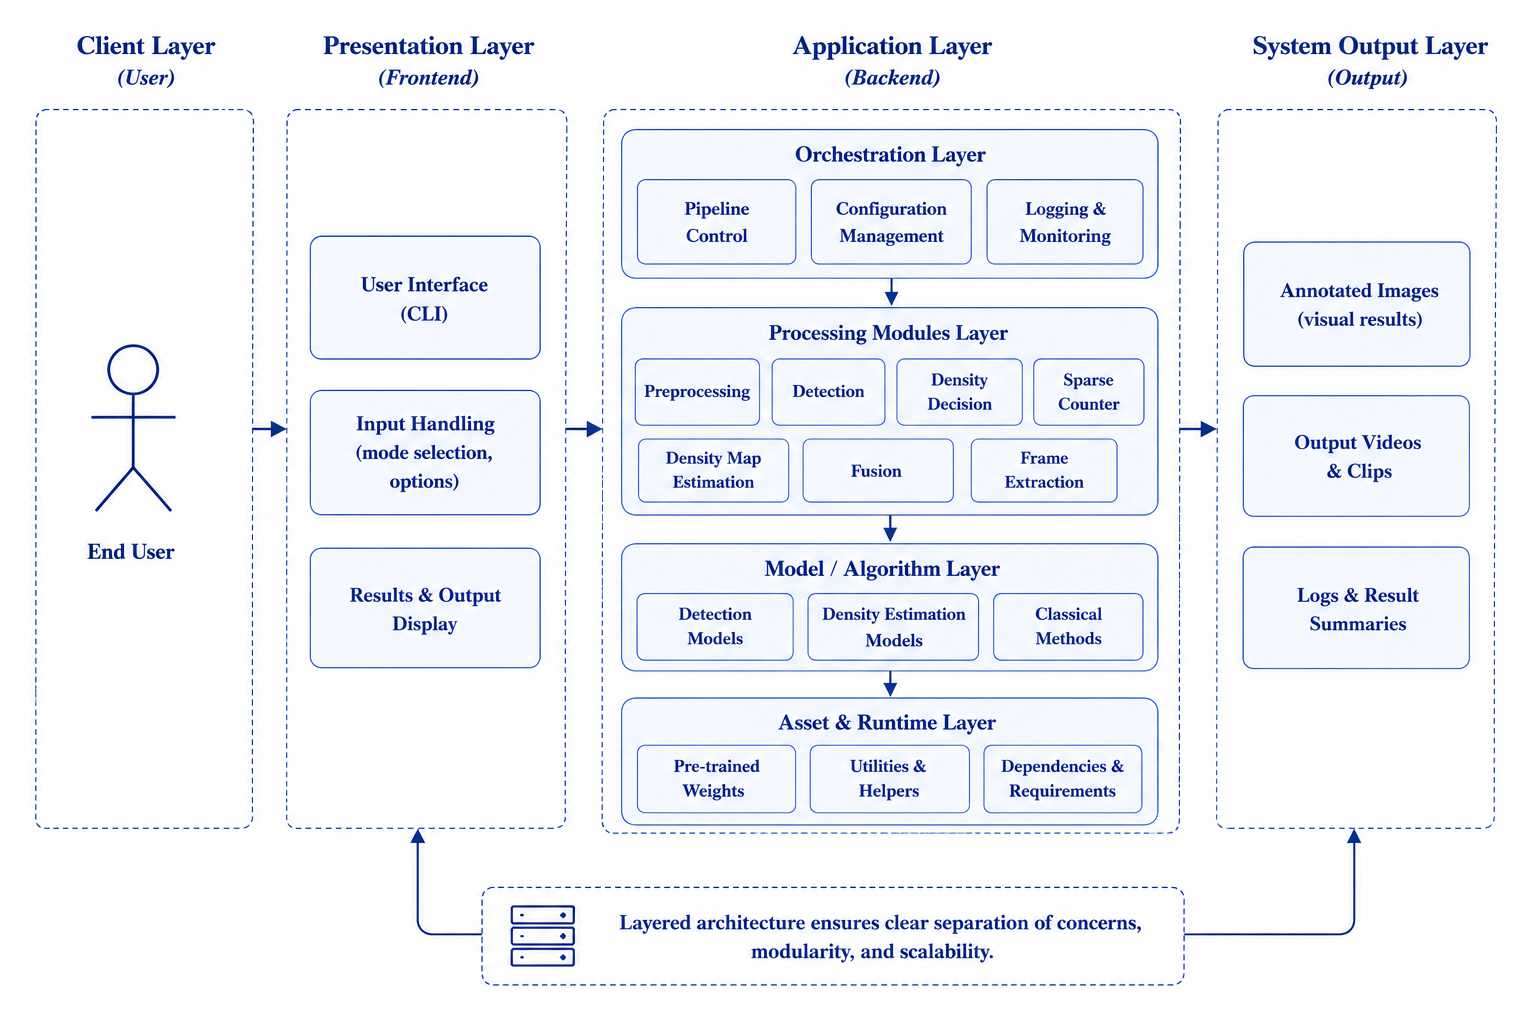
\includegraphics[width=1.0\textwidth]{./../images/system_architecture/architecture_overview.png}
    \caption{The design of the system is based on five layer architecture}
    \label{fig:archoverview}
\end{figure}

\begin{itemize}
    \item \textbf{Presentation Layer}: It reads operator input (modality and source selection), and displays the final result in the form of an annotated image or video.

    \item \textbf{Orchestration Layer}: It orchestrates the stages of processing, stores the run wide configuration and collects diagnostic and performance data for each processing stage of each run.

    \item \textbf{Processing Layer}: The processing layer consists of the following main stages: pre-processing, two parallel estimation sub-layers (sparse and dense), the scene decision and fusion logic.

    \item \textbf{Inference Layer}: The models / inferences performed by the processing layer that are trained and classical computer vision models.

    \item \textbf{Persistence Layer}: It stores for model assets, configuration and run outputs/logs.
\end{itemize}

The coupling between the levels is minimal, with high testability, for instance, the processing layer can be tested with synthetic frames in a stub configuration, without having to deploy the presentation layer or a live model asset store.

\section{High Level Design}

The system can be viewed from a high level perspective as one logical entity, which receives an image or video from an external source, and outputs an annotated image or video and a numerical annotation. The context diagram (Data Flow Diagram Level 0) for this system is shown in Figure~\ref{fig:dfd}(a) and the same system decomposed into its six constituent high level processes is a Level-1 Data Flow Diagram as shown in Figure~\ref{fig:dfd}(b).

\begin{figure}[H]
    \centering
    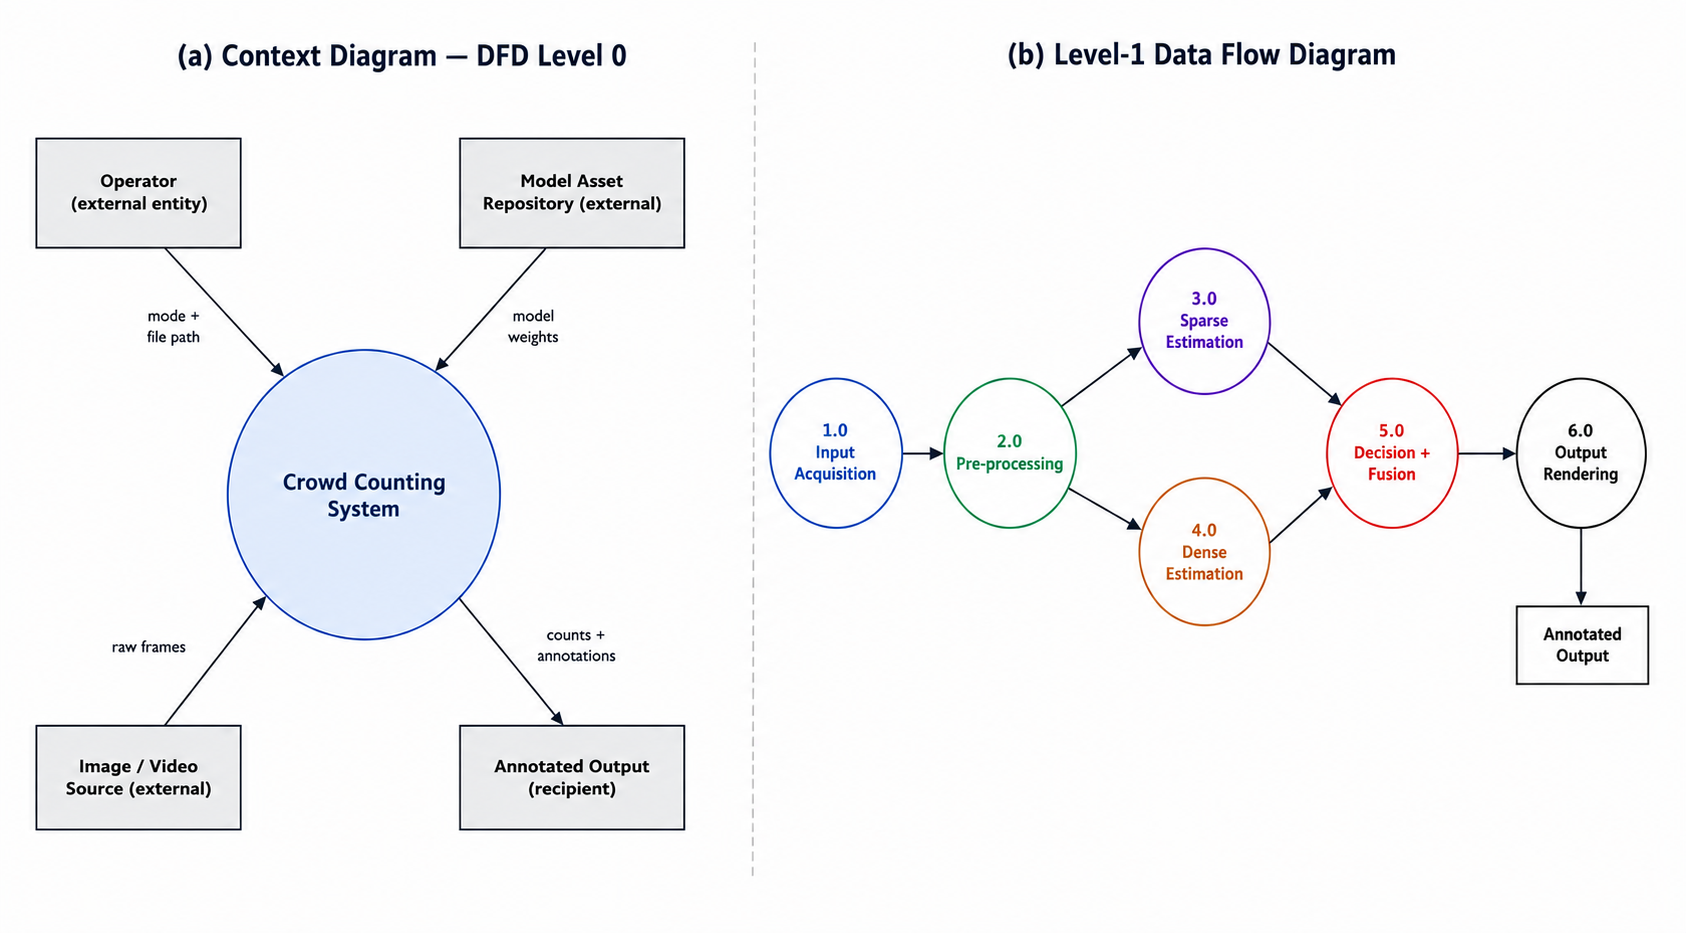
\includegraphics[width=1.00\textwidth]{./../images/system_architecture/dfd_diagram.png}
    \caption{Context Diagram \& Data Flow Diagram}
    \label{fig:dfd}
\end{figure}

The high level design was intentionally made to separate two conflicting counting strategies, sparse estimation (Process 3.0) and dense estimation (Process 4.0), into concurrent (parallel) processes where both processes read-in the same pre-processed frame and write out into a shared decision/fusion-stage (Process 5.0). The hybrid behaviour underlying the contribution of this system is a choice made when it is defined, it may be used, replaced or extended without altering the structure of the rest of the flow, because both strategies have the same abstract contract (a frame in a people count out).

Table~\ref{tab:hld-processes} summarises the responsibility of each high level process shown in the Level-1 data flow diagram.

\begin{longtable}{|
		>{\raggedright\arraybackslash}p{1.6cm}|
		>{\raggedright\arraybackslash}p{3.2cm}|
		>{\raggedright\arraybackslash}p{9.7cm}|
	}
    \caption{High-level process responsibilities (L1 DFD).}
    \label{tab:hld-processes} \\
    \hline
    \textbf{Process} & \textbf{Name} & \textbf{Responsibility} \\
    \hline
    \endfirsthead

    \hline
    \textbf{Process} & \textbf{Name} & \textbf{Responsibility} \\
    \hline
    \endhead

    1 & Input Acquisition &
    Reads a still image or samples frames from a video source at a configurable rate \\
    \hline
    
    2 & Pre-processing &
    Enhances contrast and suppresses noise before estimation \\
    \hline
    
    3 & Sparse Estimation &
    Detects discrete person/head instances in a frame, removes duplicate/overlapping detections, and reports their locations and count \\
    \hline
    
    4 & Dense Estimation &
    Estimates a continuous density map for the frame and integrates it to a count \\
    \hline
    
    5 & Decision + Fusion &
    Classifies the scene as sparse/dense and reconciles the two count estimates into a single fused count \\
    \hline
    
    6 & Output Rendering &
    Produces the annotated image/video and the numeric summary \\
    \hline

\end{longtable}

\section{Detailed Design}
\label{sec:detailed-design}

This section will provide details about the internal structure of each of the processing modules defined in the high-level design, their function, their inputs and outputs, and the main internal logic. The following module-by-module descriptions refer to the interactions that occur at runtime for a single frame, as shown in Figure~\ref{fig:sequence}.

\begin{figure}[H]
    \centering
    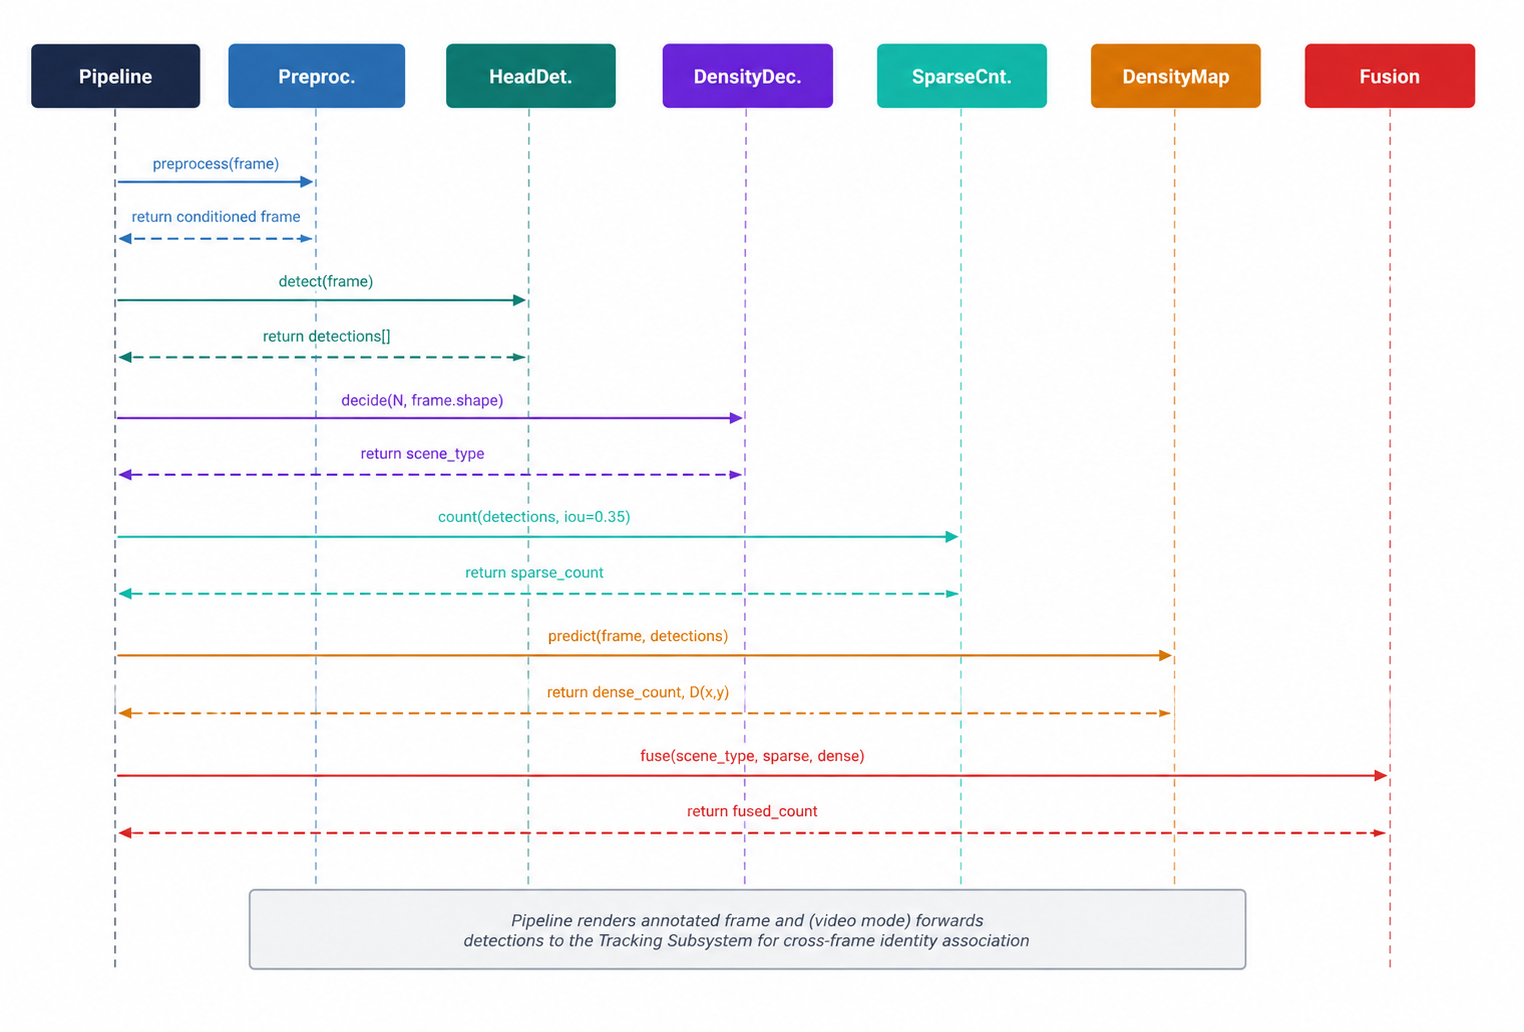
\includegraphics[width=1.00\textwidth]{./../images/system_architecture/sequence_diagram.png}
    \caption{Sequence Diagram - Single Image Processing}
    \label{fig:sequence}
\end{figure}

\subsection{Module 1: Input Acquisition}

\textbf{Responsibility:} Accepts either a still image or a video file path, checks if it is readable, and if it is a video file, does a systematic sub-sampling of temporal frames so that the rest of the stages need not process all of them.

\textbf{Input:} file path, input mode flag (image / video).

\textbf{Outputs:} One or more raw frames (as in-memory arrays) and basic metadata (resolution, time stamp and/or frame index).

\textbf{Key design decision:} The sampling interval is calculated based on the ratio of the source frame rate to a user defined target frame rate, thus allowing the module to automatically adjust when the source has different native frame rate without manual intervention from the operator.

\subsection{Module 2: Pre-processing}

\textbf{Responsibility:} Apply conditions on each raw frame to enhance the reliability of both estimation branches under uneven lighting or low lighting.

\textbf{Input:} Raw frame.

\textbf{Outputs.} A contrast enhanced frame that is slightly denoised, but otherwise the same size.

\textbf{Key design decision:} Contrast enhancement is applied to the luminance channel (not all channels) to maintain colour balance and to avoid colour artefacts that would fool the detection models.

\subsection{Module 3: Sparse Estimation}

\textbf{Responsibility:} Detects instances of persons/heads and provides a count and the location of the bounding boxes.

\textbf{Input:} The pre-processed frame.

\textbf{Outputs.} A list of confidence scores, along with a list of bounding boxes, all without duplication. A cardinality (sparse count) list.

\textbf{Key design decision.} The detector backend is abstracted by a single API and duplicate detections are avoided using the overlap based suppression step and avoiding duplicate detection because of overlapping candidate boxes from a single hand.

\subsection{Module 4: Dense Estimation}

\textbf{Responsibility:} Produces a continuous, per-pixel density estimate that is informative even if people cannot be resolved independently.

\textbf{Inputs:} The pre-processed frame.

\textbf{Outputs:} A density map and its spatial integral (the dense count).

\textbf{Key design decision:} The density estimation backend is hidden behind a single interface.

\subsection{Module 5: Decision and Fusion Unit}

\textbf{Responsibility:} Decides which of the two estimates from the branches is more reliable for a frame, and merges the two estimates to a final number.

\textbf{Input:} The detection count/locations and the density count.

\textbf{Output:} One fused count and a label of the type of scene (sparse/dense).

\textbf{Key design decision:} If the two estimates are very close, the two estimates are blended; if they are very different, the estimate from the primary branch is accepted as is, to prevent the estimate from being deflected by a silent failure in one of the branches for a particular scene type.

\subsection{Module 6: Output Rendering}

\textbf{Responsibility:} Creates the artefact visible on the operator side: Bounding boxes, optional density-map overlay, burning in the operator side the fused/unique counts.

\textbf{Inputs:} Original frame and output of all the preceding modules.

\textbf{Outputs:} An annotated image or video file.

\section{Component and Module Design}

In contrast to Section~\ref{sec:detailed-design}, which discussed the responsibilities of each module, this section discusses how each module is structurally connected to its neighbors; what interfaces each module offers for use by its neighbors; what interfaces each module requires from neighbors; and, the flow of dependency within the system. This structural view is represented by a UML component diagram as shown in Figure~\ref{fig:component}.

\begin{figure}[H]
    \centering
    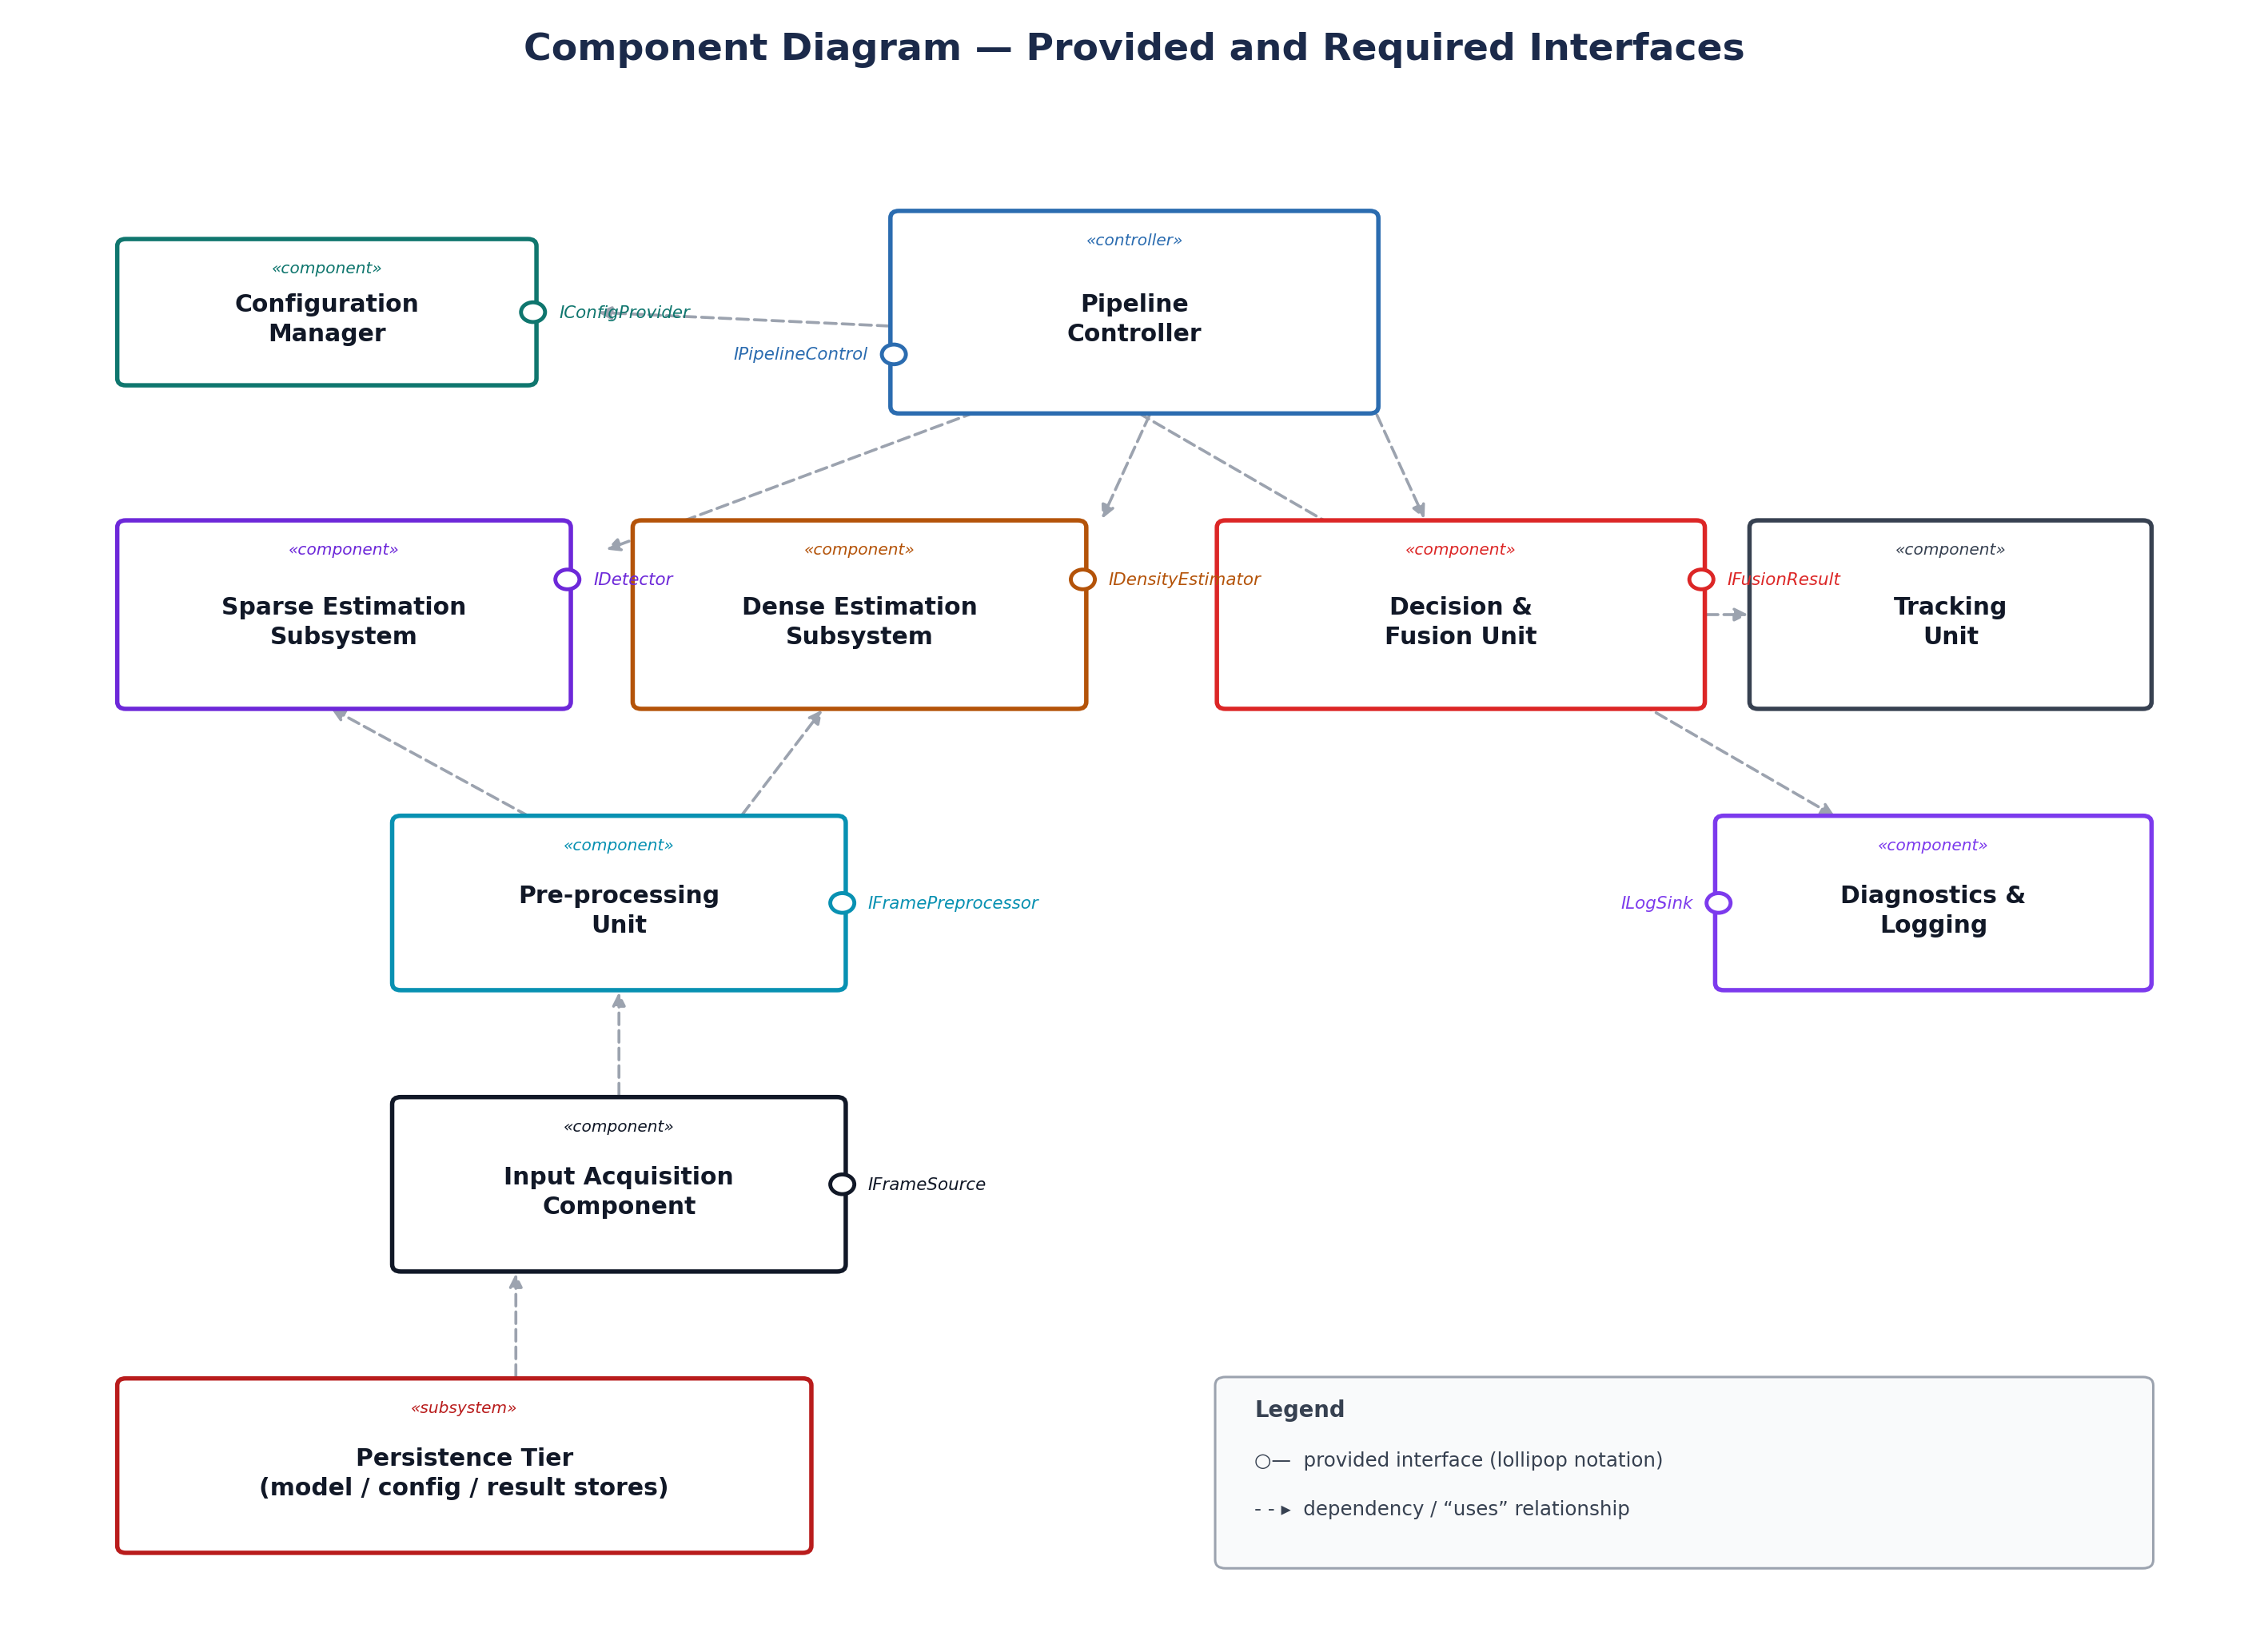
\includegraphics[width=1.00\textwidth]{./../images/system_architecture/component_diagram.png}
    \caption{Component Diagram}
    \label{fig:component}
\end{figure}

All components are built from a configuration object that is passed explicitly from outside, not from configuration or environment variables. Thus it enables independent testing of components and provides the ability to monitor the behaviour of the entire system at runtime to a single inspectable object per run.

The explicit definition of the required only relationship between the pipeline controller and the diagnostics \& logging component, shows that each component returns control to the pipeline controller between its stages, and the pipeline controller is the one that controls and times the stages and logs them. This is to ensure that there are no concerns of cross cutting such as logging out of the core estimation logic.